% ****** Start of file aipsamp.tex ******
%
%   This file is part of the AIP files in the AIP distribution for REVTeX 4.
%   Version 4.1 of REVTeX, October 2009
%
%   Copyright (c) 2009 American Institute of Physics.
%
%   See the AIP README file for restrictions and more information.
%
% TeX'ing this file requires that you have AMS-LaTeX 2.0 installed
% as well as the rest of the prerequisites for REVTeX 4.1
%
% It also requires running BibTeX. The commands are as follows:
%
%  1)  latex  aipsamp
%  2)  bibtex aipsamp
%  3)  latex  aipsamp
%  4)  latex  aipsamp
%
% Use this file as a source of example code for your aip document.
% Use the file aiptemplate.tex as a template for your document.
\documentclass[%
aip,pop,amsmath,amssymb,
%preprint,%
 reprint,%
%author-year,%
%author-numerical,%
]{revtex4-1}


\usepackage{color}
\usepackage{xcolor}
\usepackage{graphicx}% Include figure files
\usepackage{bm}% bold math
%\usepackage[mathlines]{lineno}% Enable numbering of text and display math
%\linenumbers\relax % Commence numbering lines

\newcommand{\subfigimg}[3][,]{%
  \setbox1=\hbox{\includegraphics[#1]{#3}}% Store image in box
  \leavevmode\rlap{\usebox1}% Print image
  \rlap{\hspace*{200pt}\raisebox{\dimexpr\ht1-2\baselineskip}{#2}}% Print label
  \phantom{\usebox1}% Insert appropriate spcing
}

\begin{document}

\preprint{AIP/123-QED}



\title[]{On the compressibility effect in test particle acceleration 
by magnetohydrodynamic turbulence}% Force line breaks with \\
\author{Author}
 \email{email}
 \
\affiliation{affiliation}
\author{Author}
\
\affiliation{affiliation}
\author{Author}
 \
\affiliation{affiliation}
\author{Author}
 \
\affiliation{affiliation}

%\date{\today}% It is always \today, today,
             %  but any date may be explicitly specified

\begin{abstract}
The effect of compressibility in charged particle energization by 
magnetohydrodynamic (MHD) fields
is studied in the context of test particle simulations. 
This problem is relevant 
to the solar wind and the solar corona due to the compressible 
nature of those astrophysical 
scenarios. We consider turbulent electromagnetic fields obtained from  
direct numerical simulations 
of the MHD equations with a strong background magnetic field.  
In order to explore the compressibilty effect over the particle dynamics 
we performed
different numerical experiments: an incompressible case and two weak 
compressible cases, with 
Mach number $M=0.25$ and $M=0.1$. 
We analyze the behavior of protons 
and electrons in those turbulent fields,  which are well known to form 
aligned current sheets in 
the direction of the guide magnetic field. 
We show that compressibility enhance the 
efficiency of proton acceleration and that the energization 
is due to perpendicular electric 
fields generated between currents sheets. On the other hand, 
electrons remains magnetized and 
they show an almost adiabatic motion, and no effect of compressibility 
is observed.
%Valid PACS numbers may be entered using the \verb+\pacs{#1}+ command.
\end{abstract}

%\pacs{Valid PACS appear here}% PACS, the Physics and Astronomy
                             % Classification Scheme.
%\keywords{}%Use showkeys class option if keyword
                              %display desired
\maketitle

%\begin{quotation}
%The ``lead paragraph'' is encapsulated with the \LaTeX\ 
%\verb+quotation+ environment and is formatted as a single paragraph before the first section heading. 
%(The \verb+quotation+ environment reverts to its usual meaning after the first sectioning command.) 
%Note that numbered references are allowed in the lead paragraph.
%
%The lead paragraph will only be found in an article being prepared for the journal \textit{Chaos}.
%\end{quotation}

\section{\label{sec:level1}INTRODUCTION:}
Turbulence is an ubiquitous phenomenon in many astrophysical 
environments in which a wide  
variety of temporal and spatial scales are involved. This is the case of 
the solar wind or the 
intellestar medium where the energy is transported from 
large to small scales up to 
kinetic scales where the energy is dissipated. 
Turbulence is the result of the  non linear 
interaction between fluctuations of the velocity and magnetic fields, 
leading to a 
spatial intermittency that is associated with coherent structures,
 where the dissipation is 
concentrated in strong gradient regions that impacts on the heating, 
transport and particle 
acceleration in plasma \cite{M1}.

The efficiency of MHD turbulence to accelerate charged particles 
and its importance in space 
physics has been reported by many different authors\cite{F1,L1,M2}, 
but the great variety of 
scales involved in turbulence and the particle dynamics
makes this problem a big challenge.
On long timescales (large eddy turnover times), dynamics is
governed by stochastic acceleration and momentum diffusion is
the main acceleration 
mechanism which has been mainly applied for cosmic-ray energization 
studies and frequently
addressed by quasi-linear theory (QLT)\cite{S1,CH1,Lange1}. 
In diffusion studies 
MHD turbulence is commonly represented as a random 
collection of waves, and that 
representation lacks of coherent structures that has an important role 
at particle scales\cite{Vlahos}

Dmitruk et al 2004\cite{PD1}, 
using test particle simulations in static electromagnetic fields, obtained 
from direct 
numerical simulation (DNS) of MHD equations, showed that particle 
energization at dissipation
scale is due to current sheets and the acceleration mechanism 
depends on the particle 
gyroradii. 

Using a more sophisticated model, but still static turbulent 
electromagnetic fields, Dalena et 
al 2012.\cite{Dalena2012} shows essentially the same results.
Electrons initially moving with 
Alfv\'en velocity experience parallel (to the guide magnetic field)
acceleration by 
parallel electric fields inside current sheet chanels. 
On the other hand, protons are accelerated in a two stage process: 
initially they are parallel accelerated and gain substantial energy 
in a short time. Then, when the proton gyroradius becomes
comparable with current sheet thickness,
it is accelerated perpendicularly to the guide field.  


Effects of compressible MHD on particle energization has been reported 
in diffusion studies\cite{Chandran2003,CHO1}, where supersonic
turbulence was considered.

There are also reports of test particle pitch angle scattering in 
MHD turbulence, Lynn et al 2013\cite{Lynn2013}, considering 
second order Fermi acceleration by weak compressible MHD running simultaneously
the test particle and MHD fields, and imposing a scattering rate.
It is found that compressibility 
is an important effect to produce non-thermal particles. 

Additionally, there are
studies where test particles and fields are simultaneously resolved.
Weid et al 2015\cite{Weidl2015} and Teaca et al. 2014\cite{Bogdan2014}, 
use an incompressible MHD model, analyzing the effect of the 
correlation between magnetic and velocity fields 
on pitch-angle scattering and particle 
acceleration. They found that imbalanced turbulence (nonzero cross-helicity in 
the system) enhances the particle acceleration and also 
the pitch angle scattering.

In the present work we are interested in the compressibility effect 
on particle 
acceleration by coherent structures corresponding to a direct numerical 
simulation of the MHD equations, fixing the the fields which accelerate
the particles. 
We 
analyze the particle behavior for three different situations: an 
incompressible case, and 
two weak compressible cases changing the sound Mach number value. 

The organization of this paper is the following:  In section 2  
we describe the model 
employed in our investigation, the equations and properties of 
turbulent MHD fields and the 
test particle model including the parameters that correlate 
particles and fields; 
in section 3 we show the properties of proton and electron dynamics 
and in section 4, we
discuss about our findings.

\begin{figure*}[<t>]
\begin{center}
{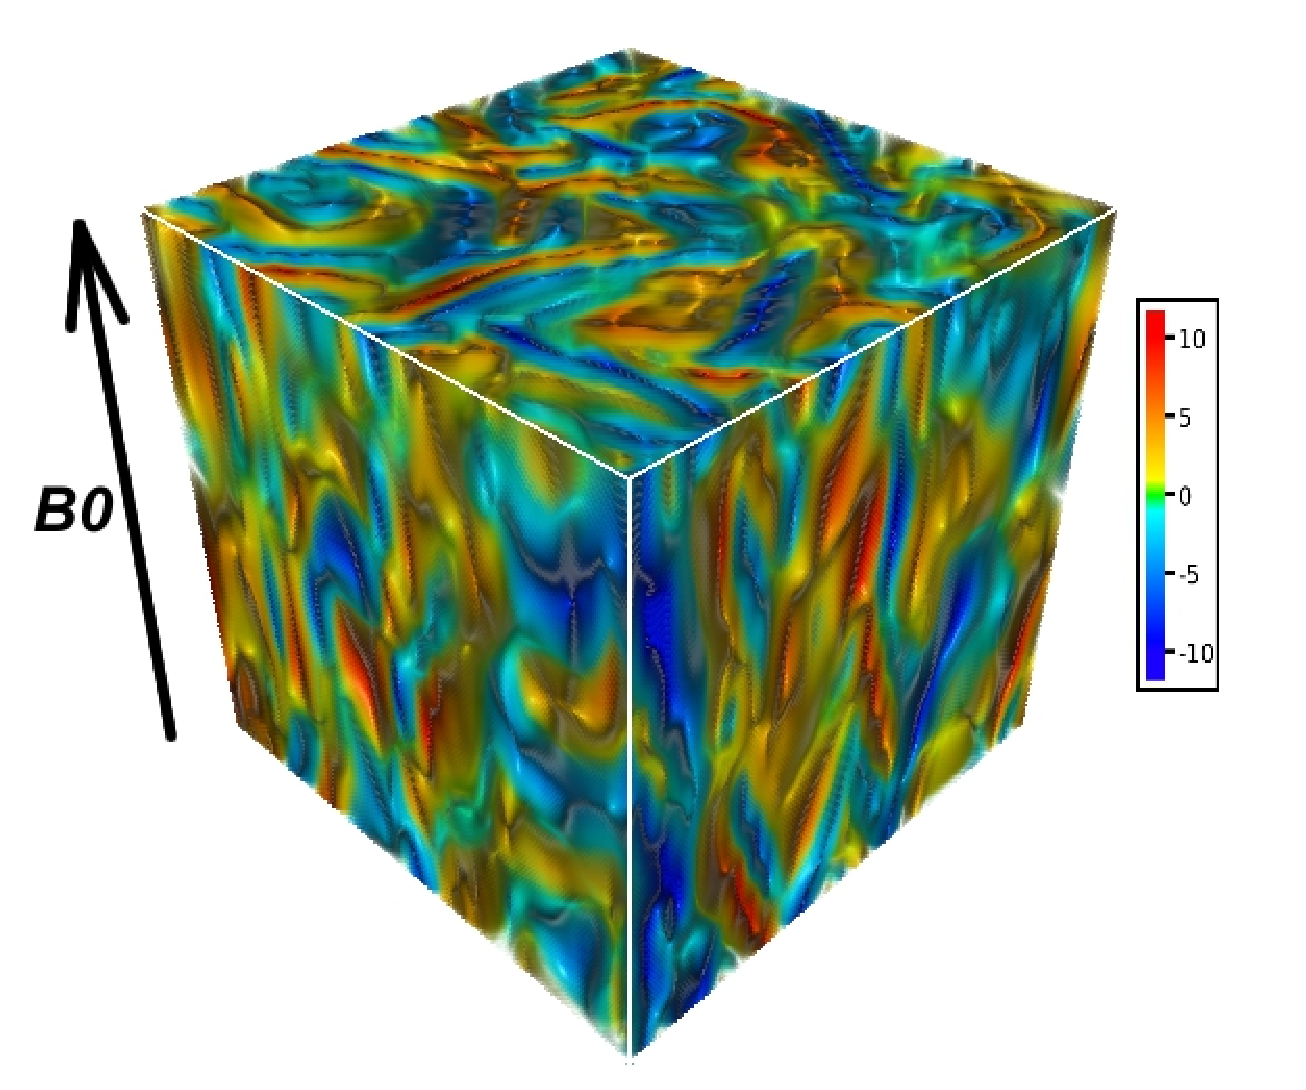
\includegraphics[width = 0.45\textwidth]{./Figures/Fig1_a}}
{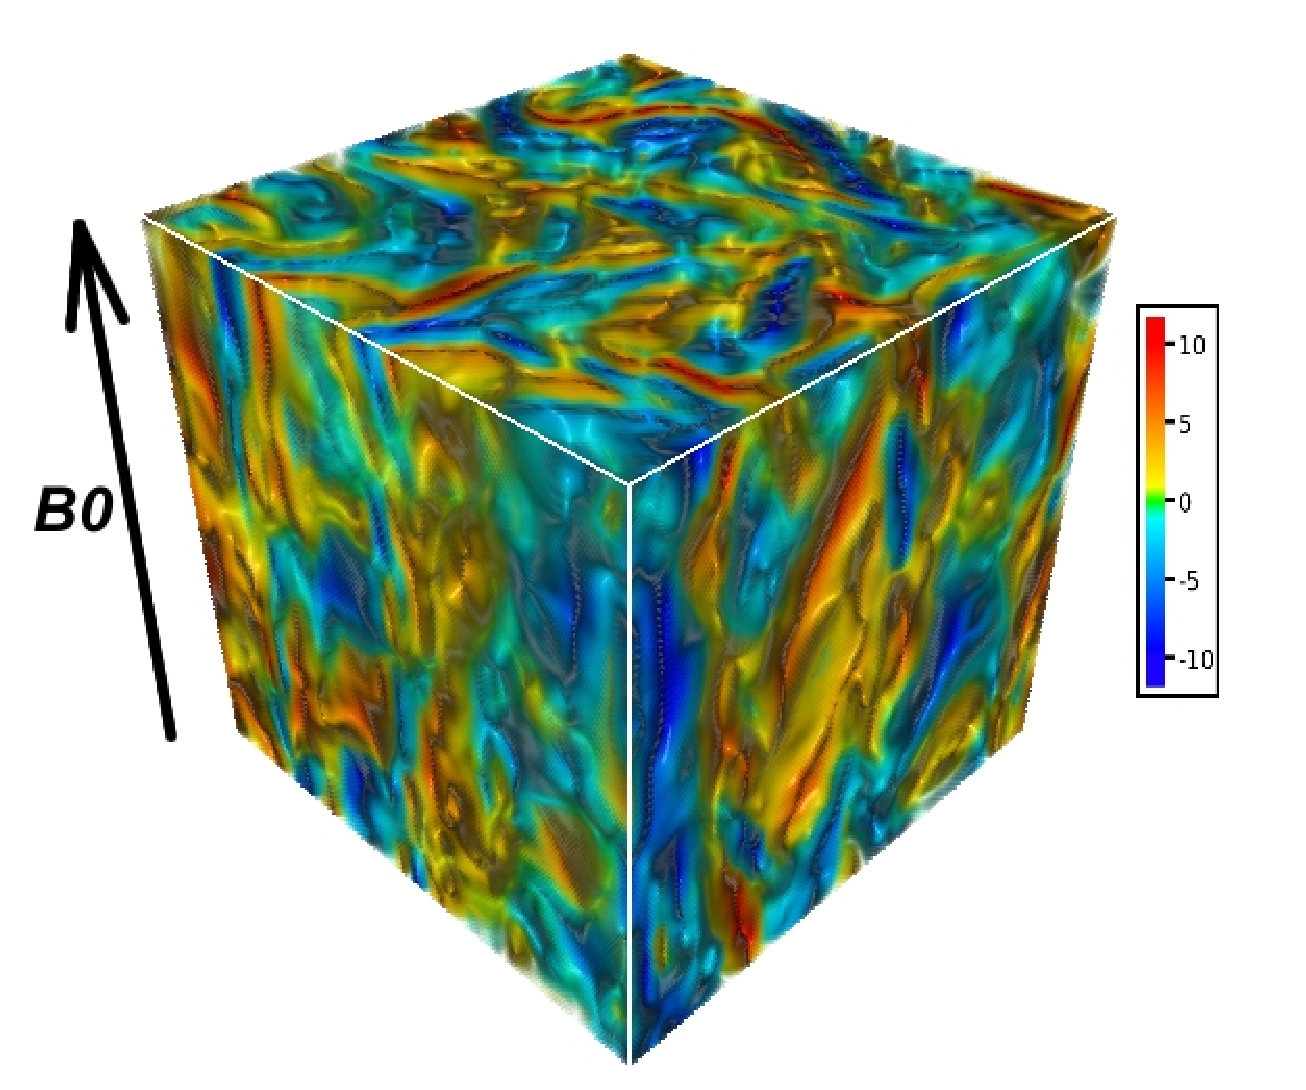
\includegraphics[width = 0.45\textwidth]{./Figures/Fig1_b}}
\caption{Three dimensional view of the parallel current density $J_z(x,y,z)$. (Left) Incompressible and 
(Right) Compressible field with Mach number $M=0.25$ case at $t/t_0 =2$.}
\end{center}
\end{figure*}


\section{\label{sec:level2}MODEL:}
The macroscopic description of a plasma is given by the three-dimensional compressible MHD equations: the continuity (density) equation, the equation of motion, the magnetic field induction equation, and the equation of state (1-4) respectively, which involves fluctuations  of the velocity field $\textbf{u}$, magnetic field $\textbf{b}$ and density $\rho$. We assume a large-scale background magnetic field $B_0$ in the z-direction, so the total magnetic field is $\mathbf{B = B_0 + b}$


\begin{equation}
 \frac{\partial \rho}{\partial t} + \nabla \cdot (\textbf{u}\rho) = 0
\end{equation}

\begin{equation}
 \frac{\partial \textbf{u}}{\partial t} + \textbf{u} \cdot \nabla \textbf{u} = - \frac{\nabla p}{\rho} + \frac{\textbf{j} \times \textbf{B}}{4\pi\rho} 
 + \nu \left( \nabla^2 \textbf{u} +    \frac{\nabla \nabla \cdot \textbf{u} }{3} \right)
\end{equation}

\begin{equation}
\frac{\partial \textbf{B}}{\partial t} = \nabla \times (\textbf{u} \times \textbf{B}) + \eta \nabla^2 \textbf{B}
\end{equation}

\begin{equation}
 \frac{p}{\rho^{\gamma}} = cte
\end{equation}


Here $p$ is the pressure, $\nu$ the viscosity, $\eta$ the magnetic 
diffusivity and
$\textbf{J}=\nabla \times \textbf{B} $ is the current density. 
We assume a polytropic 
equation of state $p/p_0= (\rho/\rho_0)^{\gamma}$, with $\gamma=5/3$, and
$p_0, \rho_0$ the equilibrium (reference) pressure and density. 
We consider two weak compressible cases with Mach number
($M= \sqrt{\gamma p/\rho}$) equal to $M=0.25$ and $M=0,1$. Additionally, 
in order to 
have a reference to measure the effect of compressibility on particle 
acceleration, we consider an
incompressible case (with $\nabla \cdot \textbf{u} = 0$).

The magnetic and velocity fields are here expressed in Alfv\'en speed units; 
a characteristic 
plasma velocity is given by the parallel Alfv\'en wave velocity
along the mean magnetic 
field $v_A = B_0/\sqrt{4\pi\rho_0}$. An Alfven speed based on field 
fluctuations can also be defined as $v_0=\sqrt{<b^2>/4\pi\rho_0}$. 
We take $v_0$ as a unit for velocity and magnetic field fluctuations. 

We use the turbulence correlation length $L$ as unit length. 
The unit timescale $t_0$
is derived from the unit length and the Alfven speed $t_0=L/v_0$.

The MHD equations are solved numerically using 
a Fourier pseudospectral method with periodic 
boundary conditions in a cube of size  $L_{box}=2\pi L$; 
this scheme ensures exact energy 
conservation for the continuous time spatially discrete equations. 
The discrete time 
integration is done with a high-order Runge-Kutta method and a
resolution of ($256^3$) 
Fourier modes is considered. For the kinematic Reynolds number 
$R=v_0L/\nu$ and magnetic Reynolds
numbers $R_m=v_0L/\eta$, 
we take $R=R_m= 1000$, which are limited here by available
spatial resolution. We consider a decaying simulation from an 
initial state with the kinetic 
and magnetic field fluctuations populating an annulus in Fourier k-space 
defined by a range of wavenumbers with
$ 3\leq k \leq4$, constant amplitudes and random phases.

When the turbulence is fully-developed a broad range of 
scales develops, from outer scale $L$ to 
dissipation scale $l_d\approx L/32$. We then consider this
turbulent (fixed) MHD state to push the test
particles.

The behavior of a test particle in an electromagnetic field 
is described by 
the nonrelativistic particle equations of motion:

\begin{equation}
  \frac{d\textbf{v}}{dt} = \alpha(\textbf{E} + \textbf{v} \times \textbf{B}), \ \ \ \  \frac{d\textbf{r}}{dt} = \textbf{v}
\end{equation}
 
The nondimensional electric field \textbf{E} is obtained from Ohm's law 
normalized with $E_0= v_0 B_0/c$ as follows:

\begin{equation}
 \textbf{E} =  -\textbf{u}  \times \textbf{B} + \frac{\textbf{j}}{R_m} 
\end{equation}

The adimensional parameter $\alpha$ relates particles and MHD field parameters:

\begin{equation}
\alpha=Z\frac{m_p}{m}\frac{L}{\rho_{ii}}
\end{equation}
Where $\rho_{ii}$ is the proton inertial length given 
by $\rho_{ii}=m_pc/(e\sqrt{4\pi\rho_0})$. The $\alpha$ parameter also 
represents the nominal 
particle gyroradii and measures the range of scales involved in the system.
One could expect a value
$\alpha \gg 1$ specially for space physics and astrophysical plasmas.
This represent a huge computational challenge due to 
numerical limitations. 
We consider here a dissipation length scale
$l_d=L/32$ as stated above, which is also of the order of
the current sheet thickness.

In the fixed MHD turbulence state, $10000$ test particles are 
randomly distributed 
in the computational box and the equation of motion of particles 
subject to the MHD
electromagnetic field are solved using a high-order Runge-Kutta method. 
Furthermore, 
we use linear interpolation for field values on each particle position.


Particles are initialized at rest but in a short time, they
acquire a Gaussian velocity distribution function with a 
root mean square (rms) value of the order of the Alfven velocity, 
as discussed in Dalena et al. 2012.
It is
well known that the particle gyroradius determines the acceleration 
process and our aim in 
this paper is to explore the compressibility effect on 
acceleration of large and small particle 
gyroradii. In the next section we show two diferent compressible cases 
with Mach number $M=0.25$ and $M=0.1$ 
and an incompressible case. In all the cases the mean magnetic field
is set to $B_0=10$. We present the behavior of protons with a 
nominal gyroradius $1/32$ and electrons  ($m_e=m_p/1836$)
with nominal gyrodadius $1/58752$.



\section{\label{sec:level3}RESULTS:}

A sketch of three-dimensional view of the z-component current density on the simulation box at
$t=2t_0$ for incompressible and compressible with $M=0.25$ is shown in the Figure 1. It is 
observed that the current sheets are aligned in the direction of the magnetic field guide, also 
it could be seen that in both cases the structures are similar but more corrugated in the 
compressible case and smoother in the incompressible one. Latter is because we used the same 
initial condition for all the simulation suited for this paper. The coherent structures like
this are presented by the natural tendency of MHD equation and the neighborhood of a sheets
is governed by others opposed sign current sheets leading to a many reconection zones, that 
is the well known to be the mechanism behind the acceleration of charged particles.

Figure 2 shows the total spectrum of kinetic (top) and magentic field (bottom) for the 
compressible $M=0.25$, $M=0.1$ and incompressible fields respectively. At inertial range
there is almost no differences between compressible and incompressible energy spectrum for 
both magnetic and velocity fields, although slightly more energy at large scales is observed
as fluid is less compressible in all cases. On the contrary, the energy contained beyond the dissipation scale 
changes for $k\geq32$, containing greater energy as Mach number increases at this scales, 
this feature is more evident in kinetic energy than in magnetic field. It is remarkable 
that protons are mostly interacting with structures with that size and it could be an 
important effect on proton acceleration.


\begin{figure}[h!]
\begin{center}
{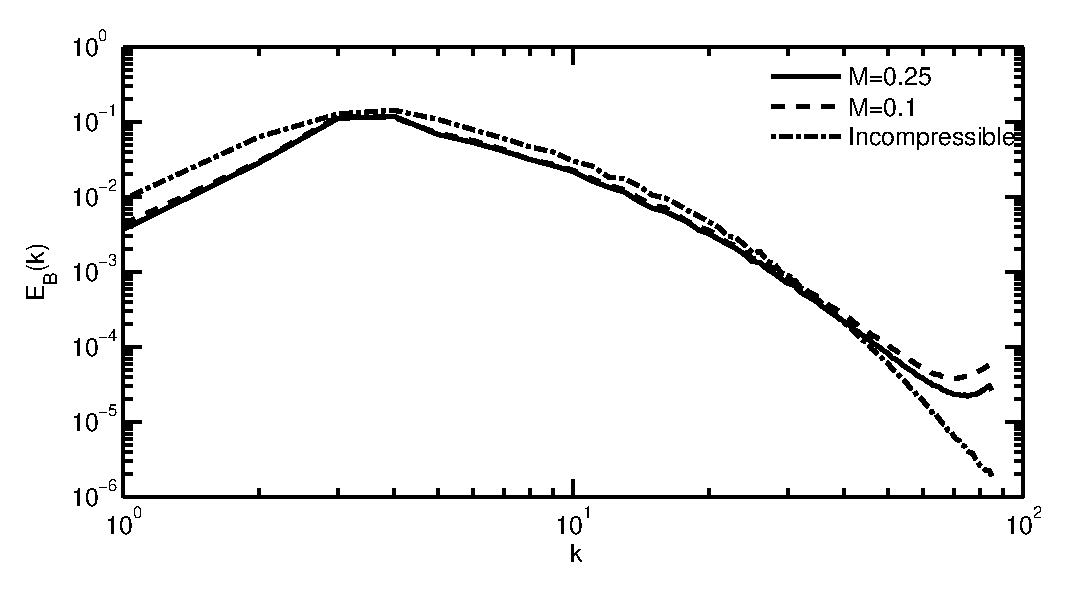
\includegraphics[width = 3in]{./Figures/Fig2_b}}\\
{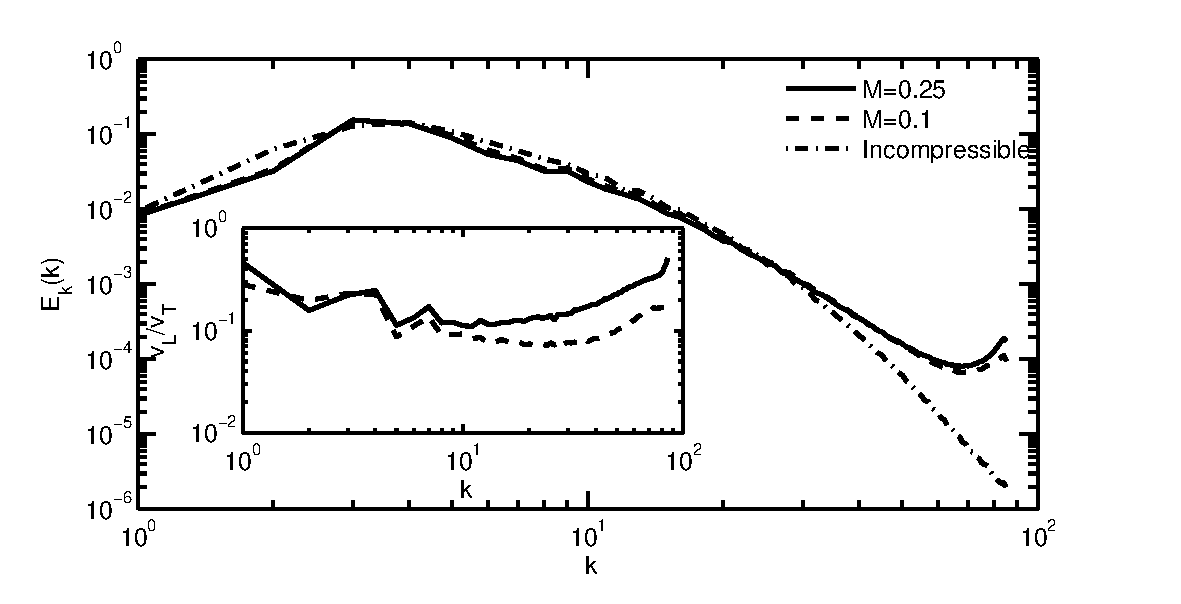
\includegraphics[width = 3in]{./Figures/Fig2_a}}
\caption{(Top). Total kinetic energy spectrum for compressible field with Mach 
number $M=0.25$ (solid line), $M=0.1$ (dashed line) and incompressible case (dashed-dot line).
(Bottom) Total Magnetic energy spectrum for the three cases named before using the same line 
type.}
\end{center}
\label{mean square velocity}
\end{figure}

The Figure 3 shows the time evolution for perpendicular $v_\perp=\sqrt{v_x^2+v_y^2}$ 
(top) and z-component of proton rms velocity (bottom) for the compressible $M=0.25$, $M=0.1$
and incompressible cases. The typical acceleration process observed in previous studies is
evident, proton are accelerated perpendicularly with respect to $B_0$, and they are less
parallel accelerated. 

Moreover, compressible effect on particle acceleration is clearly observed, on the one hand, 
protons are highly accelerated as compressibility of the fluid increases even in paralle and 
perpendicular direction, achieving almost three time higher velocity for twice Mach number value in
compressible field. Besides, the acceleration of protons in the incompressible case is less
efficiently than the compressible one, but it is also observed that protons are accelerated
but lower than in the compressible case and the value reached at the end of simulation is
shown on the inserted plot.


\begin{figure}[h!]
\begin{center}
{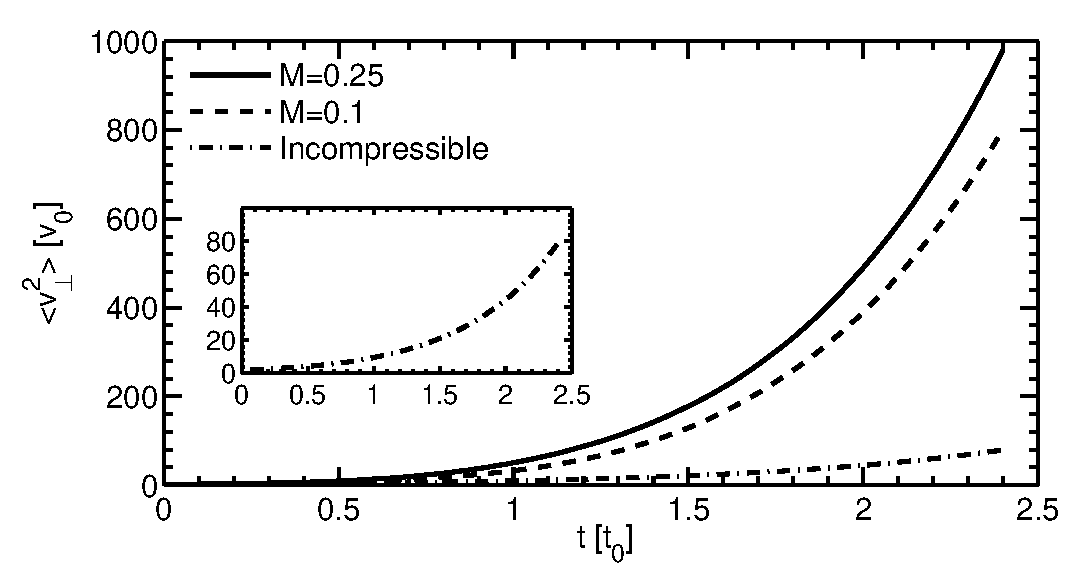
\includegraphics[width = 3.5in]{./Figures/Fig3_a}}
{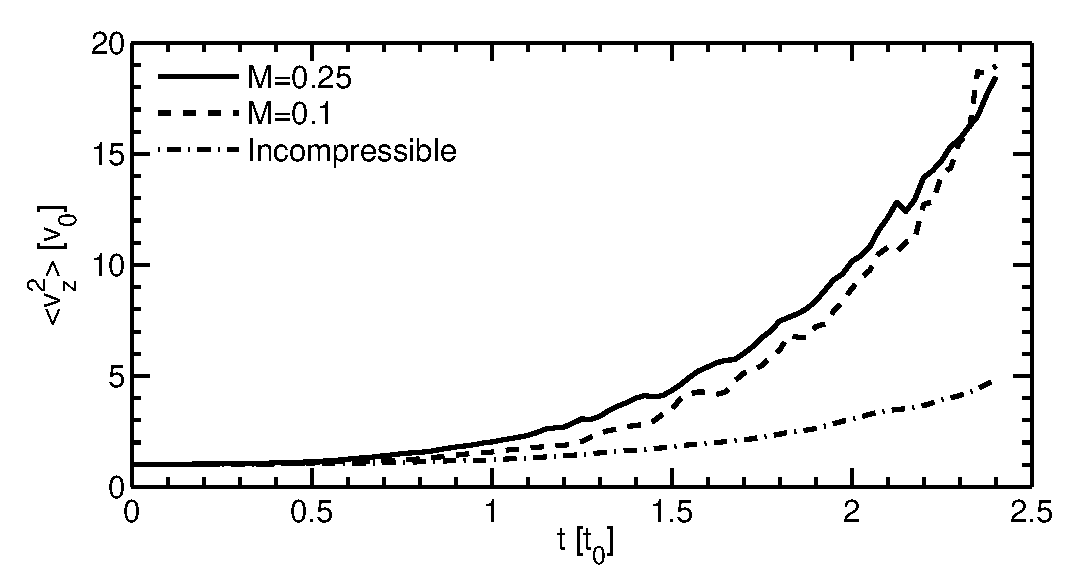
\includegraphics[width = 3.5in]{./Figures/Fig3_b}}
\caption{Particle mean square velocity as function of time in a static MHD turbulence: (Left)
Ion perpendicular velocity $v_\perp = \sqrt{v_x^2 + v_y^2}$ for two different Mach number
cases, $M=0.25$ (solid line), $M=0.1$ (dashed line) and incompressible case (dash-dot line). 
(Right) Electron parallel velocity for $M=0.25$, $M=0.1$ and incompressible field with the
same line type.}
\end{center}
\label{mean square velocity}
\end{figure}

In Figure 4 is shown a generalized view of electric field in the system, we present 
the PDF of x-component (top) and z-component of the of electric field (bottom) for 
compressible and incompressible cases. the choose of the x-component to represent the 
perpendicular electric field is not important because y-component and x-component present 
the same curve (not shown).

The perpendicular PDF shows that as compression increase long tails in the 
distribution arise and higher values of the parpendicular electric field is presented in
the simulation box, additionally the center of the distribution for incompressible case is
thicker than compressible cases, and the values between compressible cases is almost twice
higher between $M=0.1$ and $M=0.25$ cases.\\

\begin{figure}
\begin{center}
{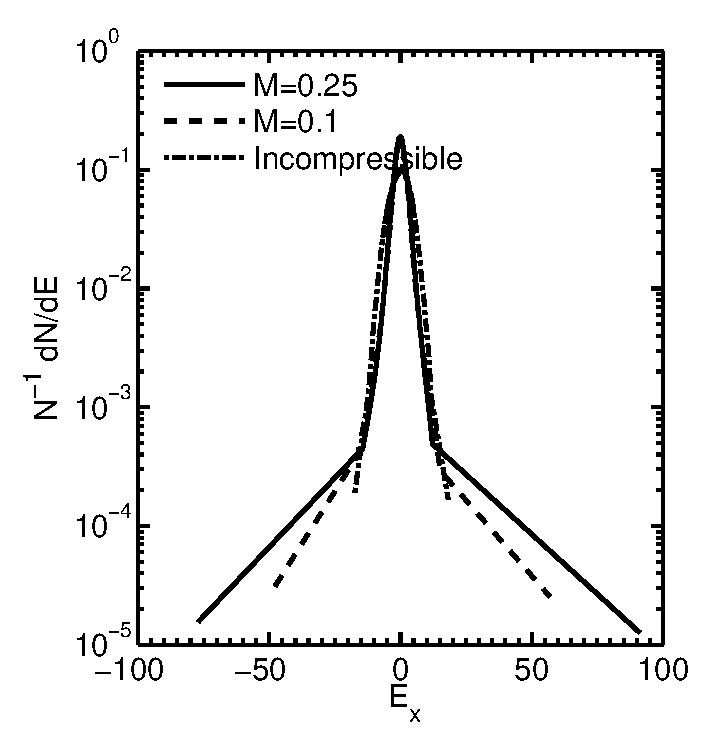
\includegraphics[width = 3in]{./Figures/Fig4_b}}
{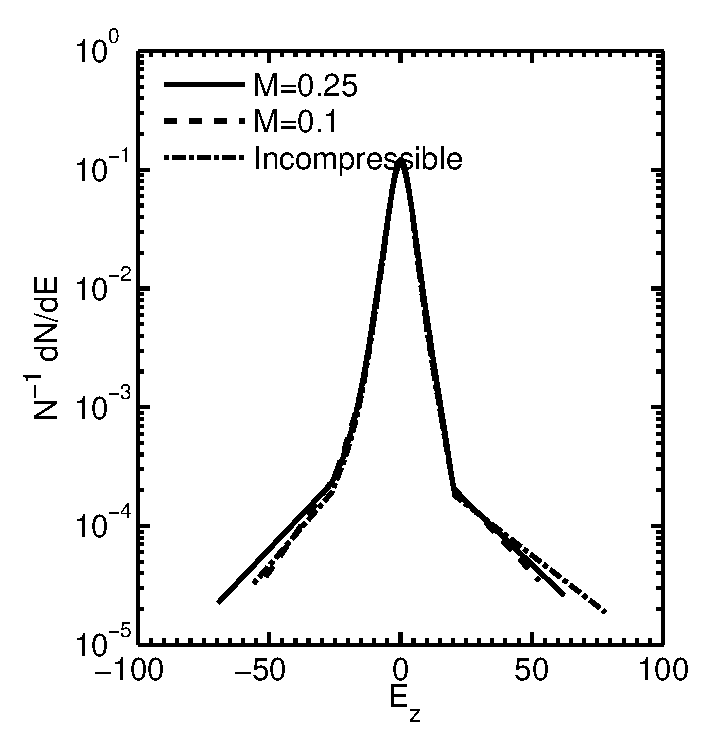
\includegraphics[width = 3in]{./Figures/Fig4_2}}
\caption{Probability density function of electric field in the simulation box. (Left) one of the 
component of perpendicular direction for $M=0.25$ (solid line), $M=0.1$ (dashed line) and incompressible field (dash-dot line). (Right) parallel component of electric field for the compressible and incompressible cases using the same line type.}
\end{center}
\label{mean square velocity}
\end{figure}
On the other hand, the PDF of parallel electric field in the system shows that there is not
effect of compression in the z-component of electric field and the values among either perpendicular
and parallel distribution are no different at all. Latter shows that perpendicular electric field is
the responsable to proton energization and in spite of the high values of parallel electric field
the parallel is lower that perpendicular energization.

In order to deeply understand the behavior of protons in that turbulent structure, In Figure
5 we show the perpendicular current desity $J_z$ on the countour of the one the most energetic protons
in the system (top) and the proton trajectory with the same box dimension (bottom) for the compressible $M=0.25$ simulation.

It is observed that on the surrounding of the particle path there are many current sheets with different 
polarity, it allows that particle encounter with the interface of opposed sheets as observed in
particle trajectory. 

\begin{figure}[h!]
\begin{center}
{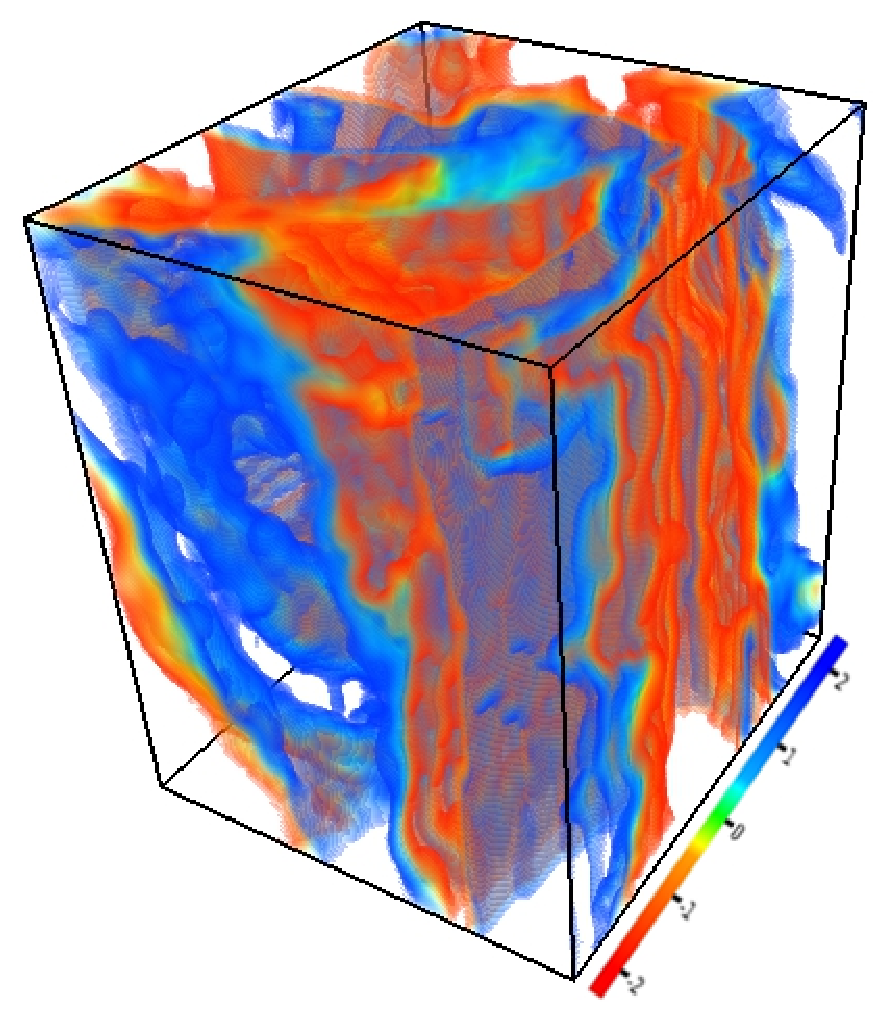
\includegraphics[width = 3in]{./Figures/Fig5_a}}
{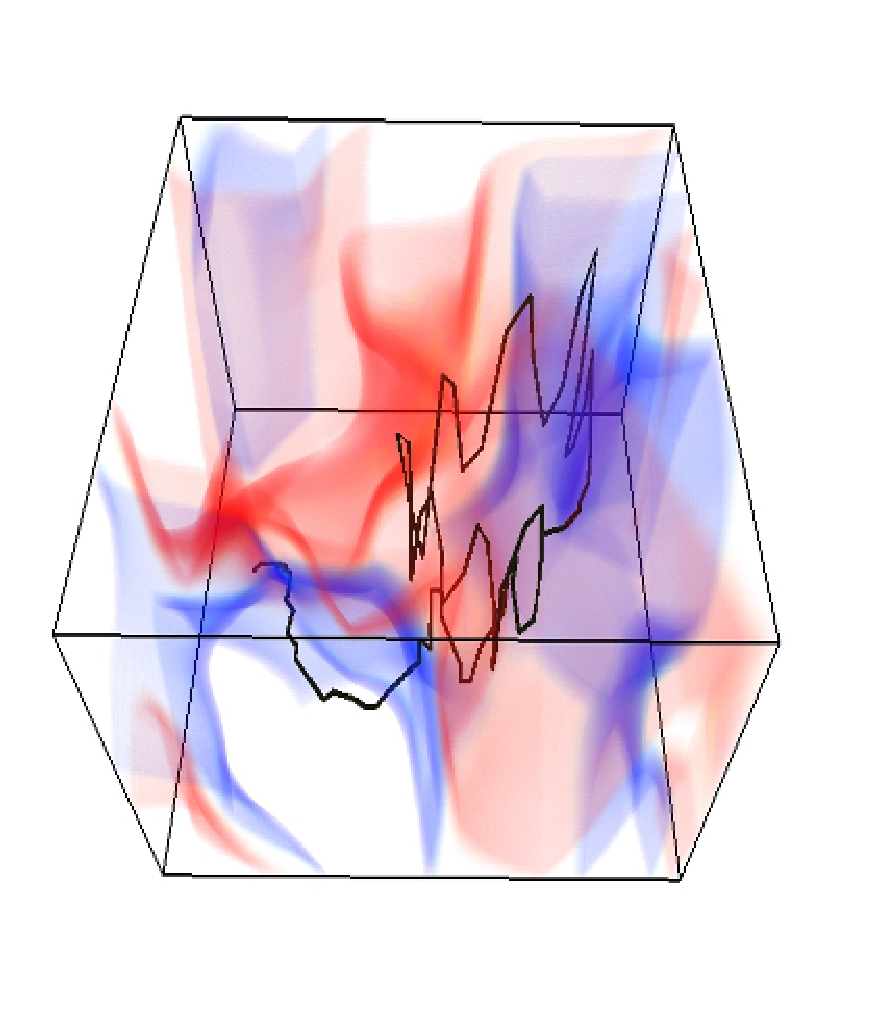
\includegraphics[height=2.87in, width = 3in]{./Figures/Fig5_b}}
\caption{Probability density function of electric field in the simulation box. (Left) one of the 
component of perpendicular direction for $M=0.25$ (solid line), $M=0.1$ (dashed line) and incompressible field (dash-dot line). (Right) parallel component of electric field for the compressible and incompressible cases using the same line type.}
\end{center}
\label{mean square velocity}
\end{figure}

\begin{figure*}[h!]
  \centering
  \begin{tabular}{@{}p{0.45\linewidth}@{\quad}p{0.45\linewidth}@{}}
    \subfigimg[width=\linewidth]{a)}{./Figures/Fig6_a_compress} &
    \subfigimg[width=\linewidth]{a)}{./Figures/Fig6_a_incompress} \\
    \subfigimg[width=\linewidth]{b)}{./Figures/Fig6_b_compress} &
    \subfigimg[width=\linewidth]{b)}{./Figures/Fig6_b_incompress} \\
    \subfigimg[width=\linewidth]{c)}{./Figures/Fig6_c_compress} &
    \subfigimg[width=\linewidth]{c)}{./Figures/Fig6_c_incompress} \\
    \subfigimg[width=\linewidth]{d)}{./Figures/Fig6_d_compress} &
    \subfigimg[width=\linewidth]{d)}{./Figures/Fig6_d_incompress}
  \end{tabular}
  \caption{(a) Parallel current density, (b) three components of the electric field, (c) velocity 
components, and (d) rms displacement as function of time for the most energetic particle in each case:
(Left) compressible $M=0.25$ field and (Right) incompressible field}
\end{figure*}

\clearpage

To explore the proton acceleration and the mechanism behind the compressible effect, we 
present in the Figure 6 the z-component of the current density (a), the electric field 
components (b), the three components of velocity (c), and the root mean square displacement 
along time (d) of the same particle sketched above on the left column and one of the most energetic
proton for the incompressible case on right column.

This temporal series of the quantities let us to know when and why protons are accelerated, it 
is clearly observed that when there is a change of the sign in the z-component of the current
density, there is also an increment in the perpendicular components of electric field that 
particle experience and concurrently there is an increment of proton velocity. This situation
is repeatedly observed in time and the energy of proton increase as it passes through that 
situation.

The change of the sign in the current density is because the particle constantly enters and 
leaves on two current sheets with different polarities, and allows particle to experience the
perpendicular electric field between current sheets. The electric field that particle measure
is stronger as compression of the fluid increases, it could be observed from the values 
reached in each case, also it could be noted that the value of electric field is independent
of the value of the current density that particle has crossed.

The velocity increments at each current sheet encounter is larger in the compression than
incompressible case, driving to a higher energy at the end of simulation for compressible case.
Latter could explain what we see in the Figure 3, where the rms perpendicular velocity of 
protons is huge for compressible case and low for incompressible one. This situation is 
generalized for many particles in the simulation which increases its perpendicular energy as
they encounter with many current sheets and then resulting in the increases of the mean 
square velocity for the ensemble of particles. 

\begin{figure}[<t>]
\begin{center}
{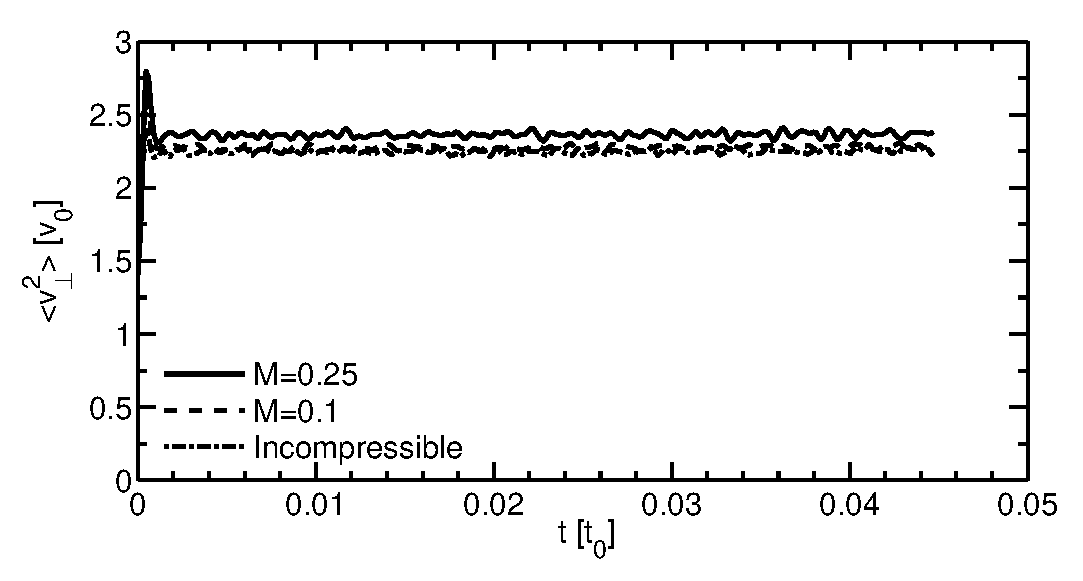
\includegraphics[width = 3.5in]{./Figures/Fig7_a}}
{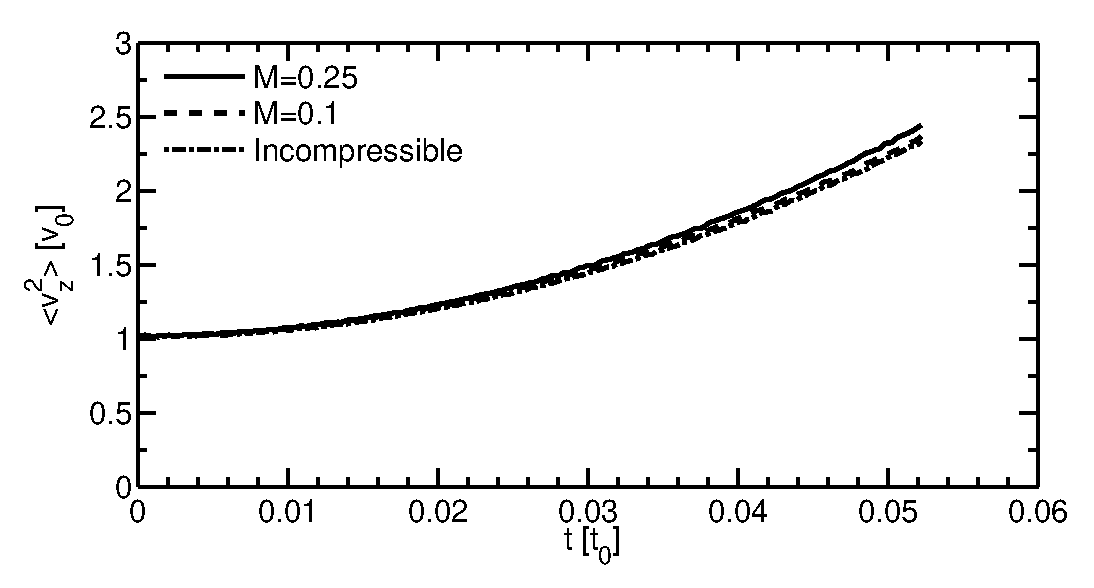
\includegraphics[width = 3.5in]{./Figures/Fig7_b}}
\caption{Probability density function of electric field in the simulation box. (Left) one of the 
component of perpendicular direction for $M=0.25$ (solid line), $M=0.1$ (dashed line) and incompressible field (dash-dot line). (Right) parallel component of electric field for the compressible and incompressible cases using the same line type.}
\end{center}
\label{mean square velocity}
\end{figure}

The Figure 7 shows the time evolution for perpendicular (top) and z-component of electron
rms velocity (bottom) for the compressible $M=0.25$, $M=0.1$ and incompressible cases.

It should be mentioned that we present a really short time simulation of electrons here
because there is a limitation in the choose of time step to ensure CFL stability condition,
and huge computational resources are needed to represent a physical fast gyroradius of real
mass electrons. The time reached in this electron simulation represents almost 3000 
electron gyroperiods which is enough to observe the typical behavior of small particle 
gyroradius.

Despite the short time simulation shown here, electrons present the typical parallel
energization reported by previous works, besides there is not evidence that compression of 
the MHD fields enhance the electron acceleration and electrons gain the same energy
regardless the compressible level of the fluid.

Instead perpendicular rms velocity shows that inially electrons are accelerated due to
their high inertia but quickly exhibit a constant perpendicular energy. Constant 
perpendicular energy is related with the magnetic momentum conservation which 
is one of the adiabatic invariance in the charged particles dynamic in a magnetic 
field, it has an enormus consequences in the dynamic of particles and determine how 
magnetized is a particle or how much trapped is a particle in a field line.

Since the gyradii of electron is smaller than any structures presented 
in the system, when electrons find a current sheet they travel forward and backward along
field lines between mirror points gaining parallel energy, and due to there is no so much 
differences between compressible and incompressible cases on z-component of electric field
the electron acceleration is not affected by compression.

It is important to state that in long timescales or the order of many turn overtimes, 
electrons could reach very high parallel energy and electrons could not still keeping 
adiabatic motion, suddenly they could reach others regions and could interact with 
structures that generate other possibles acceleration mechanisms like pitch 
angle-scattering, betatron acceleration and others.

\section{\label{sec:level4}DISCUSSION:}
We have investigated the effect of compressible MHD turbulence on particle energization 
using test particle simulation in a frozen electromagnetic field obtained from DNS of MHD
equations. We have noticed that compression affects only the energization of large particle
gyroradius or the order of dissipation length and no effect of compression for
small particle gyroradius is observed. 

Protons are accelerated by the perpendicular electric field generated on the interface of
current sheets and they gain substantial energy as they encounter these structures. 
Moreover the perpendicular electric field between current sheets is greater as compression
of the fluid increases leading to a higher proton acceleration with the compression degree.

On the other hand, small particle gyroradii keep magnetized and gain paralell energy as 
they travel along the magnetic field lines aligned with $B_0$, no compression effect is
noted for these kind of particles and that is because the compressible modes in 
magnetohydrodynamics is a perpendicular propagation mode ($k \perp B_0$) and then no
difference in the parallel electric field obtained from static MHD fields is presented.

In this paper we analyze the case of weak compressible turbulence despite the solar wind
and other astrophysical scenarios could be stronger compressible ($M \geq 1$), further we
can show that at least for low Mach number, compression could enhance the particle
energization by coherent structures and it has important implication in the study of
particle acceleration by turbulent fields.

In the incompressible case, which is the limit of infinity sound waves velocity, we 
observed that protons could be accelerated but a lesser extent than compressible case, 
and it serves as a reference to measure the influence of compression on particle 
acceleration. Also incompressible case could represent a real physical scenario like fast
solar wind which could accelerate particle as well.


Another important issue that has not been discussed on the paper is that the results do 
not depend on the resolution of the simulation. The fact that no effect of the numerical
resolution on proton energization is remarkable because the acceleration process occurs in
structures with size around  the dissipation  lenght and smaller size structures seem
to do not affect the proton energization.

\nocite{*}
\bibliographystyle{unsrtnat}
\bibliography{aipsamp}% Produces the bibliography via BibTeX.


\end{document}
%
% ****** End of file aipsamp.tex ******
